%  Kandidate prosimo, da nam posredujejo predloge za izbolj''save tega vzorca 
%  na elektronski naslov Fizikalne knji''znice: fiz.knjiz@fmf.uni-lj.si.
%---------------------------------------------------------------------------------------
%        METAPODATKI
%--------------------------------------------------------------------------------------

\begin{filecontents*}{\jobname.xmpdata}
\Title{Naslov doktorske disertacije v angleskem jeziku}
\Author{Ime in priimek}
\Keywords{disertacije\sep navodila}
\Subject{Physics}
\end{filecontents*}

%--------------------------------------------------------------------------------------

\documentclass[longbibliography,english,a4paper,12pt]{book}

\usepackage[english]{babel}    
\usepackage[utf8]{inputenc}
\usepackage{amsfonts}
\usepackage[T1]{fontenc}
\usepackage[pdftex]{graphicx}
\usepackage{fancyhdr}
\usepackage[sort, numbers]{natbib}
\usepackage{acro}

%--------------------------------------------------------------------------------------
%      DEFINICIJA AKRONIMOV
%--------------------------------------------------------------------------------------


\DeclareAcronym{FMF}{
  short            = FMF,
  long             = Fakulteta za matematiko in fiziko,
  class		= abbrev
  }

\DeclareAcronym{UL}{
  short            = UL,
  long             = Univerza v Ljubljani,
  class		= abbrev
  }

\DeclareAcronym{VIS}{
  short            = VIS,
  long             = Visokošolski informacijski sistem,
  class		= abbrev
  }

\DeclareAcronym{PACS}{
  short            = PACS,
  long             = Physics and astronomy classification scheme,
 class		= abbrev  
  }

\DeclareAcronym{pospesek}{
  short            = \bi{a},
  long             = Pospešek,
 class		= nomencl  
  }  
  
\DeclareAcronym{sila}{
  short            = \bi{F},
  long             = Sila,
  class		= nomencl  
  }    
  
  \DeclareAcronym{gostota}{
  short            = $\rho$,
  long             = Gostota,
  class		= nomencl  
  }    
  
%-----------------------------------------------------------------------------------
%     PDF/A
%----------------------------------------------------------------------------------

\usepackage{xmpincl}
\usepackage[a-1b]{pdfx} 

%------------------------------------------------------------------------------------  

\usepackage{filecontents}
\usepackage{hyperref}
\usepackage{url}
\usepackage[a4paper,inner=3.5cm,outer=2.5cm,top=2.5cm,bottom=2.5cm,pdftex]{geometry}
\usepackage[titletoc,title]{appendix}
\usepackage{epstopdf}
\usepackage{makeidx}
\pagestyle{fancy}
\setlength{\headheight}{15pt}
\usepackage{enumitem}
\usepackage{underscore}
\usepackage{tocloft}
\renewcommand{\cftpartleader}{\cftdotfill{\cftdotsep}} 
\renewcommand{\cftchapleader}{\cftdotfill{\cftdotsep}} 

\makeindex

\def\epsfg#1#2{\epsfig{file=#1.eps,width=#2}}
\def\legendamp#1#2{\vbox{\hsize=#1\caption{\small #2}}}

\setcounter{topnumber}{4}
\setcounter{bottomnumber}{4}
\setcounter{totalnumber}{5}
\renewcommand{\topfraction}{0.99}
\renewcommand{\bottomfraction}{0.99}
\renewcommand{\textfraction}{0.0}
\setlength{\tabcolsep}{10pt}
\renewcommand{\arraystretch}{1.5}

\def\bi#1{\hbox{\boldmath{$#1$}}}
\let\oldvec\vec
\def\vec#1{\mbox{\boldmath$#1$}}
\def\pol{{\textstyle{1\over2}}}
\def\svec#1{\mbox{{\scriptsize \boldmath$#1$}}}

%----------------------------------------------------------------------------------------
%    SUMNIKI
%----------------------------------------------------------------------------------------
%  Za pisanje sumnikov imamo tri moznosti:
%   --- vnasamo jih neposredno v kodnem sistemu UTF-8 (priporocljivo)
%   --- pisemo jih z latexovim ukazom, ki je namenjen natanko temu,
%       in sicer kot \v{c}, \v{s}, \v{z}, \v{C}, \v{S}, v{\Z} ali
%       malo manj pregledno kot \v c, \v s, \v z, \v C, \v S, \v Z,
%   --- pisemo jih kot "c, "s, "z, "C, "S, "Z, vendar tedaj potrebujemo
%       spodaj zapisani macro, ki znaku " pripise vlogo `izdelave' sumnika:
\catcode`\"=\active\def"#1{\v{#1}}
%       torej \v{S}krjan\v{c}ek == \v Skrjan\v cek == "Skrjan"cek
%  Pozor: narekovaj potem ne smemo vec pisati kot " ampak kot `` in ''
%       torej: "Skrjan"cek je "civkal ``"ci-"ci-"ci''.

%------------------------------------------------------------------------------------------
%   PRIPOROCILO
%
%  V primeru, da je besedilna datoteka prevelika za pregledno urejanje,
%  priporocamo, da vsebino razdelite na posamezna poglavja, ki jih v glavni
%  dokument vkljucite z ukazom \input{naslov_poglavja}.
%
%------------------------------------------------------------------------------------------

\begin{document}

%-----------------------------------------------------------------------------------------
%       NASLOVNA STRAN V ANGLESKEM JEZIKU
%----------------------------------------------------------------------------------------

\pagestyle{empty}
\begin{center}

{\large UNIVERSITY OF LJUBLJANA\\
FACULTY OF MATHEMATICS AND PHYSICS\\
DEPARTMENT OF PHYSICS\\}

\vspace{4cm}

{\Large Ime in priimek\\}

\vspace{10mm}

{\bf \Large NASLOV DOKTORSKE DISERTACIJE V ANGLE"SKEM JEZIKU}\\
\vspace{5mm}
{\sc Doctoral thesis}\\

\vfill

{\large ADVISER: Ime in priimek\\
COADVISER: Ime in priimek\\

\vspace{2cm}
Ljubljana, leto}

\end{center}

%------------------------------------------------------------------------------------------------
%       NASLOVNA STRAN V SLOVENSKEM JEZIKU
%-----------------------------------------------------------------------------------------------

\cleardoublepage
\begin{center}

{\large UNIVERZA V LJUBLJANI\\
FAKULTETA ZA MATEMATIKO IN FIZIKO\\
ODDELEK ZA FIZIKO\\}

\vspace{4cm}

{\Large Ime in priimek\\}

\vspace{10mm}

{\bf \Large NASLOV DOKTORSKE DISERTACIJE V SLOVENSKEM JEZIKU}\\
\vspace{5mm}
{\sc Doktorska disertacija}\\

\vfill

{\large MENTOR$\backslash$-ICA: naziv, Ime in priimek\\
SOMENTOR$\backslash$-ICA: naziv, Ime in priimek\\

\vspace{2cm}
Ljubljana, leto}

\end{center}
%------------------------------------------------------------------------------------------------
%        ZAHVALA (NEOBVEZNO)
%------------------------------------------------------------------------------------------------

\cleardoublepage
\mbox{}
\vfill
{\Large \bf Acknowledgements}
\vspace{1cm}\\
Na tem mestu zapi"site, komu se zahvaljujete za pomo"c pri nastanku doktorske diser\-tacije.

%-----------------------------------------------------------------------------------------------
%         IZVLECEK
%----------------------------------------------------------------------------------------------

\cleardoublepage
\foreignlanguage{slovene}{  % slovenski delilni vzorci
\begin{center}
{\bf Naslov v slovenskem jeziku}\\[3mm]
{\sc  Izvle"cek}
\end{center}
\vspace{10mm}
Kratek izvle"cek v slovenskem jeziku, do 300 besed.\\[10mm]
{\bf Klju"cne besede:}\\[3mm]
{\bf PACS:}
}


\cleardoublepage
\begin{center}
{\bf Naslov v angle"skem jeziku}\\[3mm]
{\sc  Abstract}
\end{center}
\vspace{10mm}
Kratek izvle"cek v angle"skem jeziku, do 300 besed.\\[10mm]
{\bf Keywords:}\\[3mm]
{\bf PACS:}

%---------------------------------------------------------------------------------------------------
%    KAZALO
%---------------------------------------------------------------------------------------------------

\cleardoublepage
\tableofcontents

%--------------------------------------------------------------------------------------------------
%        SEZNAM SLIK (NEOBVEZNO)
%---------------------------------------------------------------------------------------------------

\cleardoublepage\phantomsection
\renewcommand\listfigurename{List of figures}
\addcontentsline{toc}{chapter}{\listfigurename}
\listoffigures

%---------------------------------------------------------------------------------------------------
%        SEZNAM TABEL (NEOBVEZNO)
%---------------------------------------------------------------------------------------------------

\cleardoublepage\phantomsection
\renewcommand\listtablename{List of tables}
\addcontentsline{toc}{chapter}{\listtablename}
\listoftables

%--------------------------------------------------------------------------------------------------
%        SEZNAM KRATIC, SEZNAM SIMBOLOV (NEOBVEZNO)
%------------------------------------------------------------------------------------------------

\cleardoublepage\phantomsection
\chapter*{List of abbreviations and symbols}
\renewcommand\listtablename{List of abbreviations and symbols}
\addcontentsline{toc}{chapter}{\listtablename}
\printacronyms[include-classes=abbrev, name=Abbreviations]
\printacronyms[include-classes=nomencl, name=Symbols]
\cleardoublepage

%--------------------------------------------------------------------------------------------------
%       OSREDNJI DEL
%--------------------------------------------------------------------------------------------------

\pagestyle{fancy}
\fancyhead[CE,RE]{}
\fancyhead[LO,CO]{}
\fancyhead[LE]{\textbf{\nouppercase{\leftmark}}}
\fancyhead[RO]{\textbf{\nouppercase{\rightmark}}}

%\input{Introduction}
\chapter{Introduction}
\label{chInt}
Vzorec zaklju"cnega dela vsebuje najosnovnej"se elemente, ki jih lahko vklju"cimo v \LaTeX{}ov dokument. 
Ve"c o uporabi programa si lahko preberete na primer v \cite{Go}, \cite{Ba} ali \cite{Ra}. 
Na spletu je dostopna tudi "stevilna literatura v angle"skem jeziku. Dve med njimi sta \cite{ams}  in \cite{Gr}.

V tem vzorcu je za navajanje literature uporabljen program Bib\TeX. Ta je uporaben pri dalj"sem seznamu literature ali "ce avtor "zeli posamezne enote literature navesti tudi v svojih drugih delih. 
Seznam je urejen po vrstnem redu, kot se navedbe pojavijo v delu.Seznam literature se pripravi v lo"ceni datoteki in se ga zato lahko uporabi v ve"c dokumentih.


\index{Bib\TeX}

Navajanje literature pa je mo"zno tudi v okolju {\tt thebibliography}, kjer posamezne enote na"stejemo ro"cno in v poljubnem vrstnem redu.

V poglavju~\ref{chVse} je navedena vsebina zaklju"cnega dela, ki je razvidna tudi iz strukture te predloge.
Poglavje~\ref{chMa} opisuje vstavljanje matemati"cnih izrazov in ena"cb ter sklicevanje na ena"cbe. 
Poglavje~\ref{chSl} vsebuje slike in tabele, podnaslavljanje ter sklicevanje na njih.
Poglavje~\ref{chOdd} je namenjeno informacijam o oddaji dela v tiskani obliki, oddaji v \ac{VIS} in ustreznem formatu zaklju"cnega dela.


%\input{Vsebina dela}
\chapter{Vsebina dela}
\label{chVse}

Zelo pomemben je jezik ter razumljivost pisanja. Besedilo mora biti pripravljeno v skladu s pravili za objavo v znanstveni reviji. 
Nekaj koristnih nasvetov o strokovnem pisanju najdete v "clanku prof. Ivana Ku"s"cerja : O strokovnem pisanju \cite{Ku}. 
Pomagate si lahko tudi z navodili Ameri"skega fizikalnega dru"stva \cite{APS}.\\

Vse strani morajo biti "stete, tudi prazne strani, priloge med besedilom in na koncu dela. 
Osrednje besedilo mora biti o"stevil"ceno z arabskimi "stevilkami, za"cetne in kon"cne strani pa so lahko o"stevil"cene tudi z rimskimi "stevilkami. 
"Stevilke morajo biti izpisane na spodnjem delu strani. Tisk naj bo razen za"cetnih strani dvostranski. Velikost "crk naj bo 12 pt., razmak med vrsticami pa enojen. 
Obvezna je vezava v trde platnice.\\

{\bf Vrstni red vsebine:}

\begin{itemize}[noitemsep]
\item{Naslovna stran v angle"skem jeziku}
\item{Naslovna stran v slovenskem jeziku}
\item{Izjava o avtorstvu, istovetnosti tiskane in elektronske verzije doktorske diser\-tacije in objavi osebnih podatkov "studenta, z lastnoro"cnim podpisom.
Stran z izjavo ni "steta in je vsebovana samo v tiskanem delu.}
\item{Zahvala (neobvezno)}
\item{Izvle"cek v slovenskem jeziku. Dodajte tudi klju"cne besede v slovenskem jeziku in stvarne vrstilce po  \href{http://physics.zju.edu.cn/pw/ymdm/file/pacs/pacs.html}{\ac{PACS}}}
\item{Izvle"cek v angle"skem jeziku. Dodajte tudi klju"cne besede v angle"skem jeziku in stvarne vrstilce po  \href{http://physics.zju.edu.cn/pw/ymdm/file/pacs/pacs.html}{\ac{PACS}}}
\item{Kazalo vsebine}
\item{Kazalo slik, kazalo tabel, kazalo kratic (neobvezno)}
\item{Uvod}
\item{Osrednji del}
\item{Zaklju"cni del}
\item{Seznam literature}
\item{Dodatki (neobvezno)}
\item{Raz"sirjeni povzetek v slovenskem jeziku (vsaj 10 strani)}
\item{Stvarno kazalo (neobvezno)}
\item{Seznam objav ("ce obstajajo)}
\end{itemize}

Literatura mora biti citirana "ze v besedilu. Citirani viri sproti povedo, kje naj bralec i"s"ce dodatne informacije. 
Seznam naj bo urejen po vrstnem redu, kot se navedbe pojavijo v delu. 
V primeru uporabe programa {Bib\TeX} za navajanje lite\-rature izberite Bib\TeX{ov} stil, prirejen po apsrev4-2.bst, ki ga najdete na spletni strani poleg te predloge. 
Navodila za delo s programom {Bib\TeX} najdete na spletni strani \cite{Bib}, navodila za namestitev paketa REVTeX 4.1 pa na strani \cite{Rev}. 
Za vnos bibliografskih enot priporo"camo uporabo programa \href{http://www.jabref.org/}{JabRef} \cite{JR}. 
V sezamu literature te predloge smo naslove spletnih strani in online dokumentov vnesli v polje {\tt URL}. "Ce "zelite, da se vam v seznamu literature elektronski naslov izpi"se,
ga vnesite v polje {\tt Note} pred datumom ogleda spletne strani.
Pred izpolnjevanjem polj obvezno preberite navodila v pomo"ci (JabRef help). Tu je izsek iz navodil: \href{https://help.jabref.org/en/Bibtex}{About bibtex} \cite{Help}.\\

\index{Bib\TeX}

Seznam objav je seznam va"sih "clankov, ki so bili "ze objavljeni ali so sprejeti v objavo. 
Vsebina "clankov mora biti povezana z vsebino doktorske disertacije in prav je, da se na njih v disertaciji vsaj enkrat sklicujete. 
Zato so navedeni tudi v seznamu literature. V tej predlogi so kot primeri lastnih "clankov izbrani "clanki \cite{Multiple}, \cite{Variation} in \cite{Diffusion}. 
Zaradi enostavnej"sega vnosa smo za njihovo navajanje uporabili okolje {\tt enumerate}.


%\input{Matemati"cni izrazi}
\chapter{Matemati"cni izrazi}
\label{chMa}

Spodnje besedilo je izsek iz u"cbenika J.~Strnada \cite{St}, kjer na straneh 35 in 36 navaja Newtonove zakone gibanja:

\section{Osnovne ena"cbe gibanja}
\subsection{Newtonovi zakoni}

Pri poskusih ugotovimo, da se giblje telo, na katerega deluje konstantna sila, enakomer\-no pospe"seno. 
Enaka sila povzro"ci vedno enak pospe"sek danega telesa.  
Ugotovitve pri poskusih in druge izku"snje izrazimo z Newtonovimi zakoni~\footnote{~Zakone je objavil Isaac Newton 1687 v knjigi {\it Principia mathematica philosophiae naturalis.}  Prvi zakon je poznal "ze Galileo Galilei, ki ga je objavil 1638.}:

\begin{enumerate}
\item{Telo miruje ali se giblje premo enakomerno, "ce ne deluje nanj nobena sila.}
\item{Pospe"sek je sorazmeren s silo in ima smer sile.}
\item{"Ce deluje prvo telo na drugo telo s silo, deluje drugo telo na prvo z nasprotno enako silo.}
\end{enumerate}

Tretji zakon je znan kot zakon o vzajemnem u"cinku (zakon o akciji in reakciji).
Drugi zakon zapi"semo z ena"cbo

\begin{equation}
{\bi F} = m {\bi a} \> .
\label{1NZ}
\end{equation}

\ac{sila} je vektor, saj ima poleg velikosti tudi smer. 
\ac{pospesek} je vzporeden z vektorjem sile. 
Sorazmernostni koeficient  $m$ je masa.  To je koli"cina, ki meri vztrajnost telesa pri pospe"sevanju. 
Masa je v zvezi z mno"zino snovi.  Opazovanja in poskusi ka"zejo, da je masa aditivna: 
masa $m$ telesa, ki ga sestavimo iz telesa z maso $m_1$ in telesa z maso $m_2$, je enaka vsoti obeh mas:
$$
m = m_1 + m_2 \>.
$$
V Newtonovem zakonu (\ref{1NZ}) ne smemo videti definicije za silo ali definicije za maso. 
To je zakon narave, ki ga izlu"s"cimo iz opazovanj in poskusov. 

%\input{Slike in tabele}
\chapter{Slike in tabele}
\label{chSl}

Slike in dalj"se tabele praviloma vklju"cujemo v dokument kot plavajo"ce objekte ali plovke (angle"sko floats).
Polo"zaj plovke v kon"cnem izdelku je odvisen od poteka besedila.
"Ce "zelimo dolo"citi to"cno mesto plovke, ukazu \verb|\begin{figure}|
ali \\ \verb|\begin{table}| dodamo [dolo"cilo]:

\begin{itemize}
\item[---]{{\tt h} \hspace{1 cm} tukaj}
\item[---]{{\tt t} \hspace{1 cm} na vrhu strani}
\item[---]{{\tt b} \hspace{1 cm} na dnu strani}
\item[---]{{\tt p} \hspace{1 cm} na posebni strani}
\end{itemize}

\noindent
Uporabljene slike in tabele morajo biti opremljene s podnaslovi s "cim ve"cjo pojasnjevalno vrednostjo. 
Pazite na upo"stevanje dolo"cil avtorskega prava. Pri povzetih slikah ali tabelah mora biti poleg naslova naveden tudi vir in na"cin pridobitve dovoljenja za uporabo v primeru, ko je bilo to potrebno. 
Vir slike ali tabele vklju"cite v seznam literature.

\begin{figure}[h]
\begin{center}
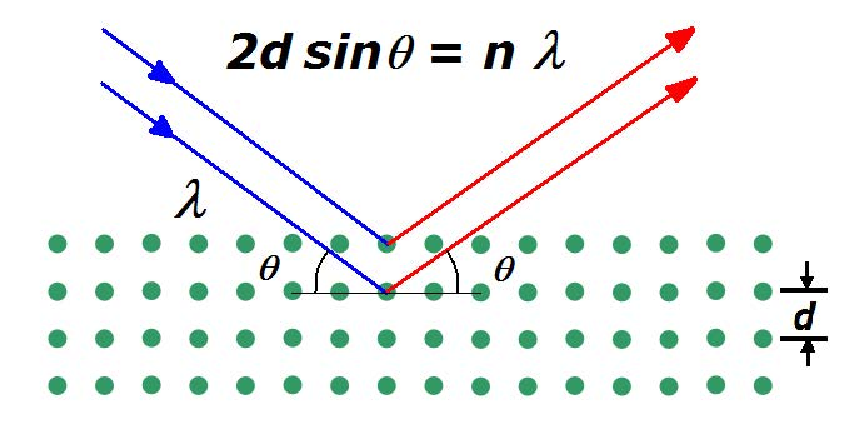
\includegraphics[width=10cm]{Bragglaw}
\end{center}
\caption[Braggov uklon.]{Braggov uklon je uklon oziroma sipanje rentgenskih "zarkov na kristalni mre"zi. 
Pri tem pride v dolo"cenih smereh zaradi interference do mo"cnih oja"canj. Slika je povzeta iz \cite{Bragg}.}
\label{pic1}
\end{figure}

\index{plovke}

Zaklju"cno delo lahko vsebuje kazalo slik in kazalo tabel. 
"Ce je podnapis predolg, da bi ga vklju"cili v kazalo, lahko namesto njega z ukazom \verb|\caption[...]{...}| med oglatima oklepajema navedemo [skraj"sani podnapis], s katerim se bo slika ali tabela pojavila v kazalu.

\newpage
\section{Formati slik}

V \LaTeX{}ov dokument lahko vklju"cimo slike razli"cnih formatov. 
Vedeti pa moramo, da program {\tt pdflatex} podpira ve"c formatov kot {\tt latex}. 
Pri uporabi programa {\tt latex} lahko vstavljamo slike edino v formatu PostScript (.ps ali .eps). 
"Ce uporabljamo {\tt pdflatex}, so primerni formati na primer .png, .pdf in .jpg.  
Tudi slike v formatu .eps je mo"zno vstaviti, "ce tako kot v tem vzorcu uporabimo paket {\tt epstopdf}, ki vsako .eps sliko samodejno pretvori v obliko .pdf.  
(Lahko pa seveda vsako .ps in .eps sliko "ze prej sami pretvorimo v sliko formata .pdf z istim programom in uporabljamo le .pdf slike.  
To je morda celo najbolj priporo"cljiva pot.)  
Strnjeno v Tabeli~\ref{tbl1}.

\begin{table}[h]
\caption[Dovoljeni formati slik]{Mimogrede: napisi k slikam so {\sl pod\/} slikami, 
napisi k tabelam so {\sl nad\/} tableami.  Ta tabela prikazuje
dovoljene formate slik.}
\label{tbl1}
\begin{center}
\begin{tabular}{l|ccc}
format & {\tt latex}  & {\tt pdflatex} \\ \hline
.pdf & ne  & da  \\
.png & ne  & da  \\
.jpg & ne & da  \\
.eps & da & da, pretvorjen z {\tt epstopdf} \\
.ps & da & da, pretvorjen z {\tt epstopdf}  \\
.bmp & ne & ne \\
.gif & ne & ne 
\end{tabular}
\end{center}
\end{table}

Pogosta te"zava, zaradi katere dokumenta ni mogo"ce pretvoriti v zahtevani format PDF/A-1b, je transparentnost slik. 
Transparentnost morate odstraniti, preden sliko vklju"cite v dokument. 

%\input{Oddaja dela}
\chapter{Oddaja dela}
\label{chOdd}

V skladu s Pravilnikom o zaklju"cnih delih "studentov \acs{UL} \acs{FMF}, sprejetim 9. 11. 2016, 
izpolnite Izjavo o avtorstvu, istovetnosti tiskane in elektronske verzije doktorske di\-sertacije in objavi osebnih podatkov "studenta
(ustvarite jo v sistemu \acs{VIS} (Zaklju"cek "studija / Izjava ob oddaji dela)).
Izjavo natisnite, podpi"site in jo uve"zite v vse tiskane izvode doktorske disertacije, kot je navedeno v poglavju ~\ref{chVse}. 
Tiskano delo oddajte v "studentsko pisarno v sedmih izvodih. V primeru, da imate pri pripravi dela somentorja, delo oddajte v osmih izvodih. 
Obvezna je vezava v trde platnice.

\section{Platnice in hrbet}

Pri izdelavi platnic upo"stevajte postavitev besedila, kot je prikazano na Sliki \ref{pic2}.

\begin{figure}[h]
\begin{center}
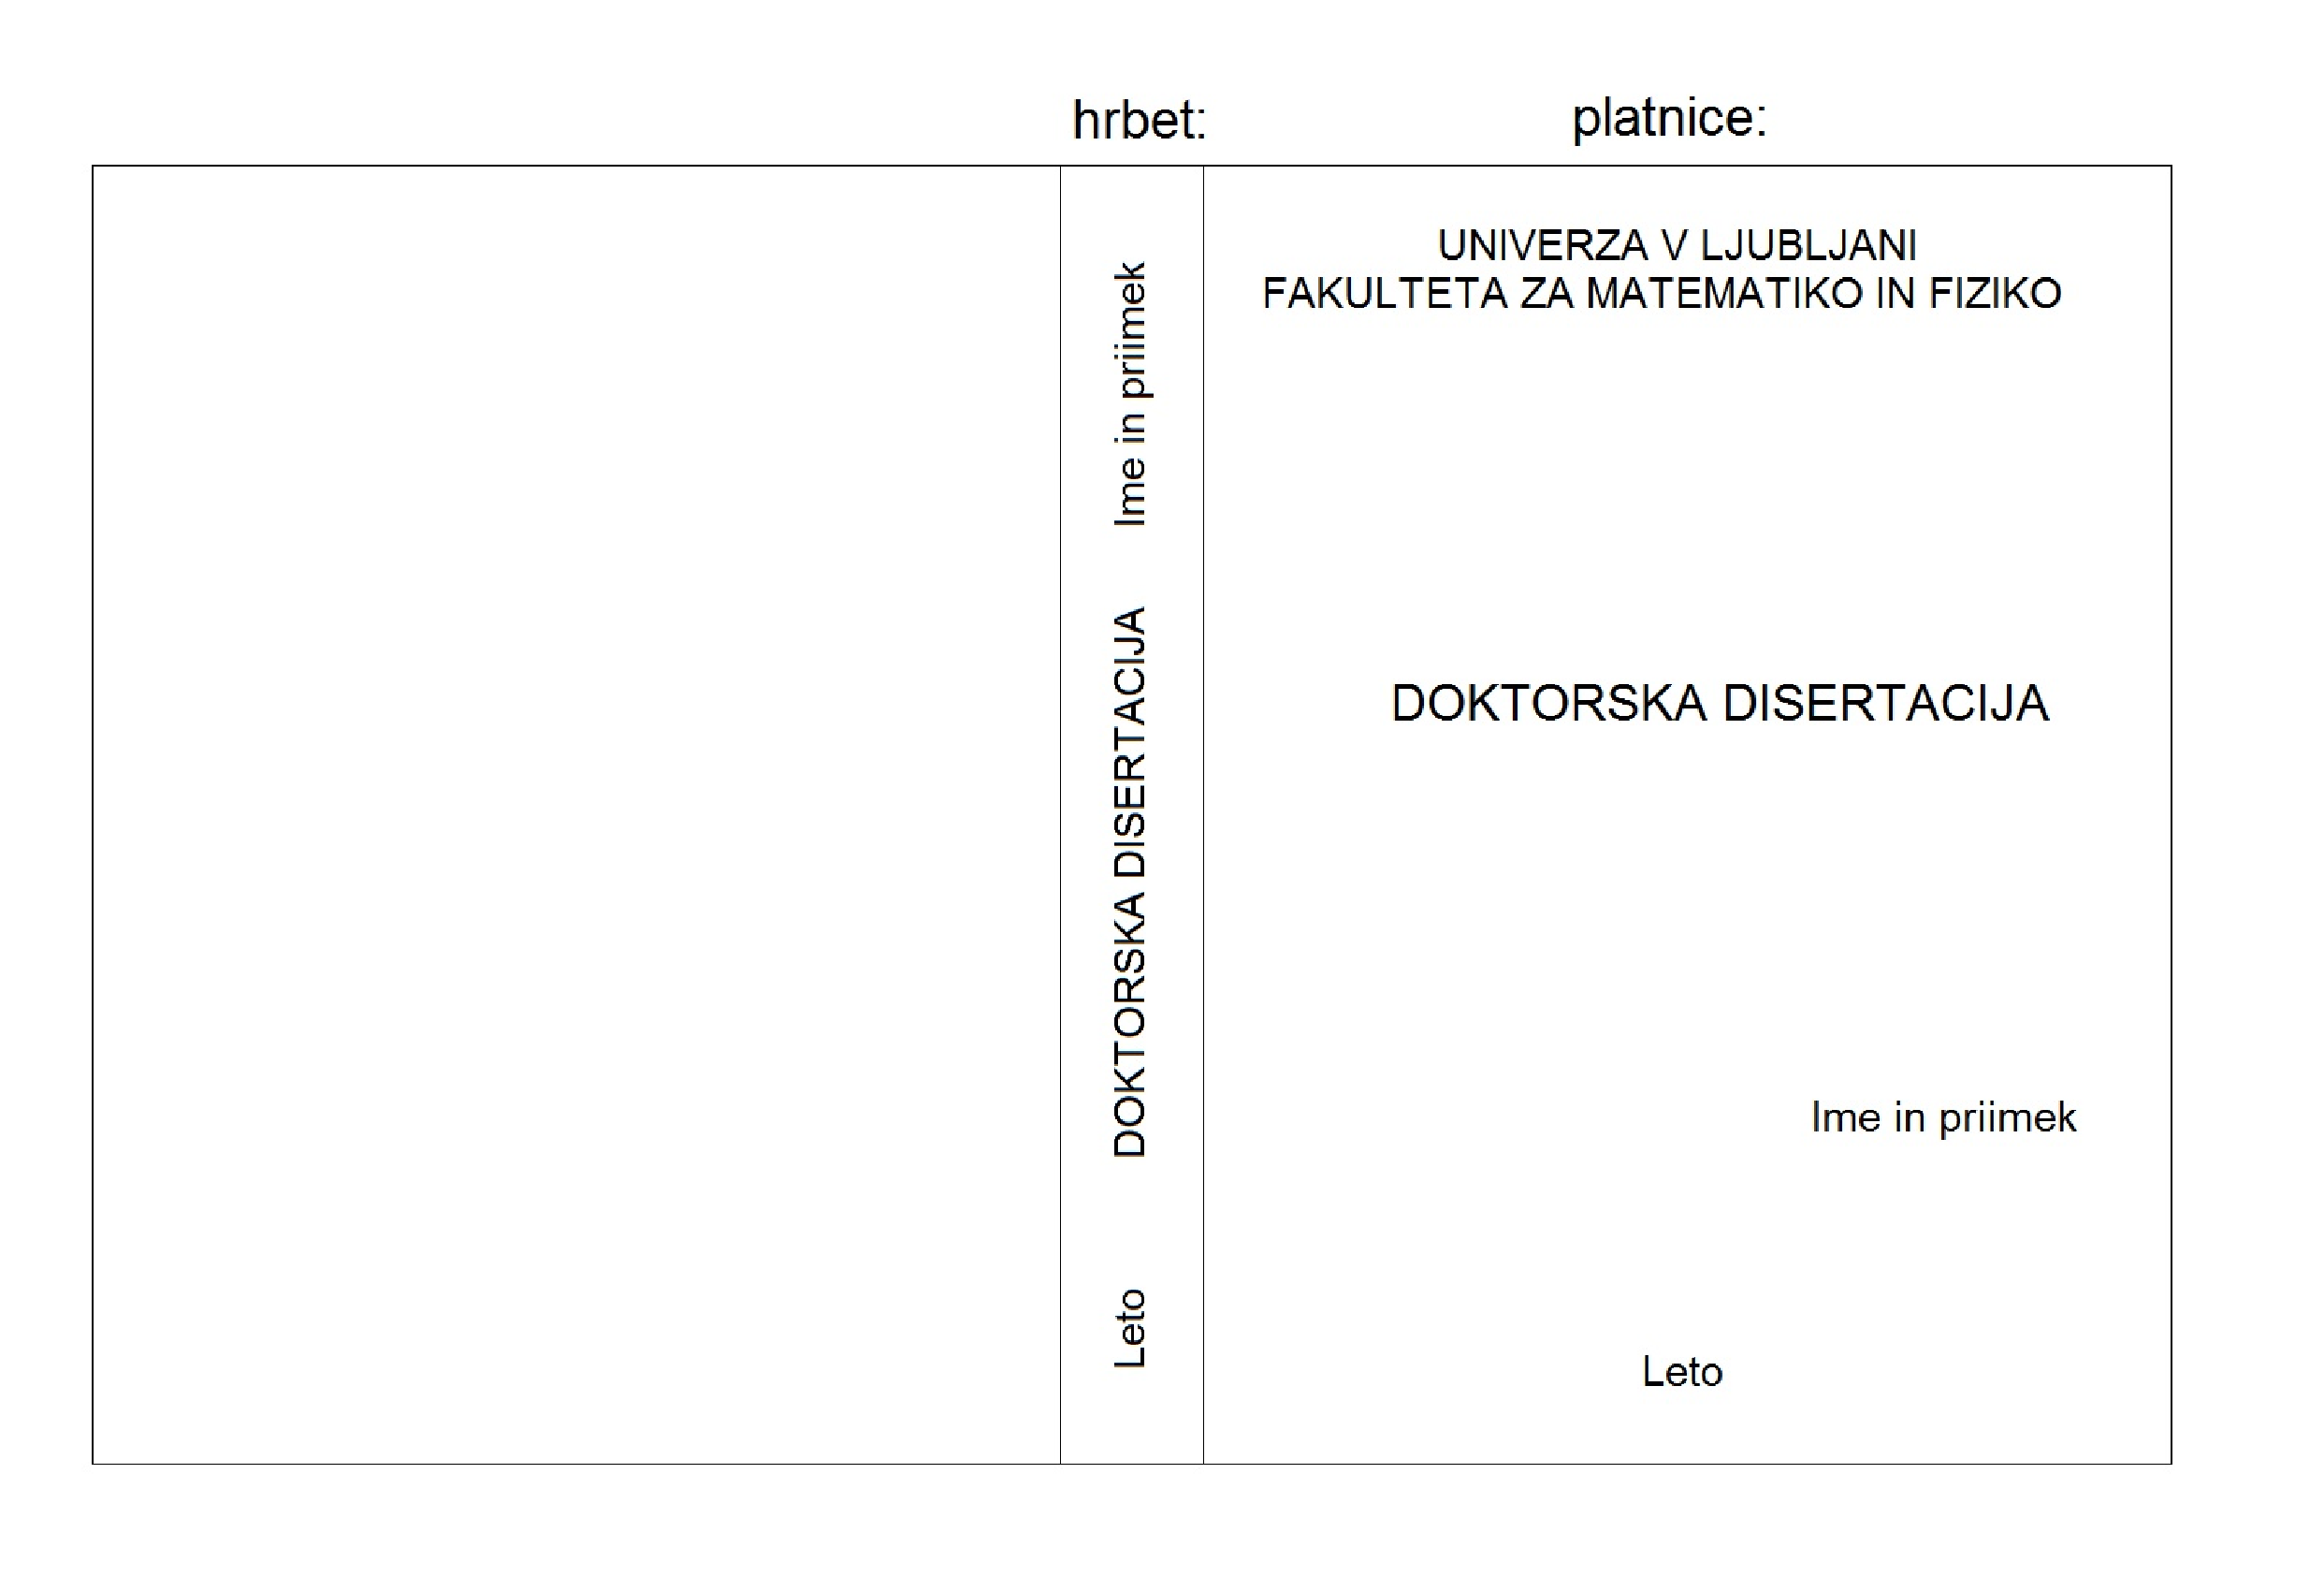
\includegraphics[width=15cm]{Platnicedoktorat}
\end{center}
\caption[Platnice]{Postavitev besedila na platnicah in hrbtu disertacije}
\label{pic2}
\end{figure}

Pred oddajo doktorske disertacije v VIS po"sljite pdf disertacije v tehni"cni pregled na elektronski naslov fizikalne knji"znice: \href{mailto:fiz.knjiz@fmf.uni-lj.si}{fiz.knjiz@fmf.uni-lj.si}.
Delo morate oddati preko sistema \acs{VIS} v preverjanje podobnosti in v hrambo Repozitorija \acs{UL}. 
Samo preverjanje podobnosti lahko traja tudi nekaj dni, zato oddajte svoje delo v sistem \acs{VIS} pravo"casno. 
Pri tem so vam lahko v pomo"c navodila: Oddaja elektronskih oblik pisnih zaklju"cnih del "studija in preverjanje podobnosti vsebine na Univerzi v Ljubljani: navodila za "studente \cite{Oddaja}.
Pri vnosu dela pazite na popolno ujemanje vnesenega naslova z naslovom v elektronski in tiskani verziji. 
Elektronska in tiskana verzija dela morata biti identi"cni. 
V sistemu \acs{VIS} je v vse rubrike mo"zno vna"sati matemati"cne simbole, kot so vneseni v \LaTeX{ovi} besedilni datoteki. 
Najve"cja mo"zna velikost datoteke je 50 MB, enaka omejitev velja tudi za priloge. Oddano delo mora biti v PDF/A-1b formatu. 

\section{Izdelava zaklju"cnega dela v formatu PDF/A-1b}

\index{PDF/A-1b}

Izdelava datoteke, ki ustreza standardu PDF/A-1b, je mo"zna na dva na"cina:\\

\noindent
1. Neposredno iz \LaTeX{ove} besedilne datoteke\\
2. Posredno iz obi"cajnega dokumenta v PDF obliki\\

\begin{enumerate}
\item{\bf Izdelava neposredno iz \LaTeX{ove} besedilne datoteke:}

Za uspe"sno generiranje PDF/A datoteke potrebujete naslednje pakete, ki so v novej"sih razli"cicah \LaTeX{a} (pdfTeX 1.40.15 ali kasnej"si) "ze vklju"ceni: pdflatex, hyperref, xmpincl in pdfx.

"Ce ustreznih datotek za delo "se nimate, si v mapo z \LaTeX{ovimi} datotekami prekopirajte naslednje datoteke, ki jih najdete na spletni strani poleg te predloge:

\noindent
{\it 8bit.def,\\
 glyphtounicode-cmr.tex,\\
 pdfa.xmp, \\
pdfx.sty} in \\
{\it sRGB_IEC61966-2-1_black_scaled.icc.}\\

Na za"cetku besedilne datoteke vnesite metapodatke o va"sem delu: naslov, avtor, klju"cne besede. 
Slike, ki jih vklju"cujete v dokument, ne smejo biti transparentne.

Po zagonu pdflatex-a se samodejno generira datoteka s kon"cnico .xmpdata, ki vsebuje metapodatke. Ker se datoteka pri ponovnem zagonu pdflatex-a "cez staro ne prepi"se, jo je potrebno v primeru spremenjenih metapodatkov prej brisati.\\

Ustvarjeno PDF datoteko odprite in jo z ukazom ``shrani kot'' ponovno shranite. V pomo"c pri delu so vam lahko spletne strani:\\
\href{http://www.mathstat.dal.ca/~selinger/pdfa/}{Creating high-quality PDF/A documents using LaTeX}\cite{Se},\\
\href{https://tug.org/tug2015/preprints/moore-pdfx.pdf}{Generation of PDF/X and PDF/A compliant PDF's with PDFTEX - pdfx.sty} \cite{Moo} ali 
\href{https://blog.zhaw.ch/icclab/creating-pdfa-documents-for-long-term-archiving}{Creating PDF/A Documents for Long-Term Archiving} \cite{Zhaw}.\\

\item{\bf  Izdelava posredno iz obi"cajnega dokumenta v PDF obliki}

\index{PDF/A-1b}

Pred pretvarjanjem v PDF/A-1b v dokument vnesite metapodatke.

Zaklju"cno delo v PDF/A-1b formatu lahko generirate s pomo"cjo programa Adobe Acrobat Pro, ki je name"s"cen na ra"cunalniku v knji"znici:

Tools -> Print Production -> Preflight -> Convert to PDF/A-1b

ali z enim izmed brezpla"cnih programov, ki jih najdete na spletu.

Preverjanje ustreznosti dokumenta (ne glede na na"cin izdelave):

V pregledovalniku PDF datoteke preverite, ali va"sa datoteka vsebuje prave metapodatke.

Preverite, ali va"sa PDF datoteka ustreza PDF/A-1b standardu, tako da uporabite enega izmed spletnih validatorjev, npr.\\
\url{https://www.pdf-online.com/osa/validate.aspx} \cite{Val},\\
ali uporabite funkcijo Preflight v programu Adobe Acrobat Pro.

"Ce pri izdelavi svojega zaklju"cnega dela v PDF/A obliki potrebujete pomo"c, lahko poi"s"cete nasvet v Fizikalni knji"znici.

\end{enumerate}

%\input{Conclusion}
\chapter{Conclusion}

Pisanje zaklju"cnega dela od vas zahteva veliko truda. Lotite se ga z veseljem, ob morebitnih vpra"sanjih ali te"zavah pa smo vam na voljo zaposleni na Oddelku za fiziko.


%------------------------------------------------------------------------------------
%       LITERATURA
%------------------------------------------------------------------------------------

\cleardoublepage\phantomsection
\renewcommand\bibname{Bibliography}
\addcontentsline{toc}{chapter}{Bibliography}
\bibliographystyle{apsrev4-2-fmf-eng}
\bibliography{Bibliografija-eng}


%-------------------------------------------------------------------------------------
%       DODATKI
%------------------------------------------------------------------------------------

\cleardoublepage\phantomsection
\renewcommand\appendixname{Appendix}
\begin{appendices}

%\input{Naslov prvega dodatka}
\chapter{Naslov prvega dodatka}
    
Dodatek je samostojna vsebina, ki ne sodi v osrednji del besedila. 
Ima svoj naslov in pravilno je, da se nanj v besedilu vsaj enkrat sklicujemo.
V dodatek spadajo na primer zahtevnej"se izpeljave, dalj"se tabele ali seznami ter vsebine, ki niso neposredno povezane z osrednjim besedilom. 
"Ce je dodatkov ve"c, jih ozna"cimo s "crkami: Appendix A, Appendix B itd.

%\input{Naslov drugega dodatk}
\chapter{Naslov drugega dodatka}
    
V pomo"c pri pisanju znanstvenega besedila vam je lahko na primer knjiga \cite{All}.

\end{appendices}


\cleardoublepage\phantomsection
\addcontentsline{toc}{chapter}{Raz"sirjeni povzetek v slovenskem jeziku}
\chapter*{Raz"sirjeni povzetek v slovenskem jeziku}
\markboth{Raz"sirjeni povzetek v slovenskem jeziku}{}

\foreignlanguage{slovene}{  % slovenski delilni vzorci
Raz"sirjeni povzetek v slovenskem jeziku naj bo dolg vsaj 10 strani. 
Vklju"cuje naj tudi slike, tabele in ena"cbe, ki so nujne za razumevanje besedila povzetka.
}

%---------------------------------------------------------------------------------
%       KAZALO (NEOBVEZNO)
%--------------------------------------------------------------------------------

\cleardoublepage
\printindex

%------------------------------------------------------------------------------
%       SEZNAM OBJAV (CE OBSTAJAJO)
%-----------------------------------------------------------------------------

\cleardoublepage\phantomsection
\addcontentsline{toc}{chapter}{List of publications related to this doctoral thesis}
\chapter*{List of publications related to this doctoral thesis}


\begin{enumerate}

\item
Ivan Ku"s"cer,
\textit{Multiple small-angle scattering of light},
Prog. Nucl. Energy
\textbf{34},
355 (1999).

\item
E. J. Van Duijn, G. Nienhuis, L. J. F. Hermans, I. Ku"s"cer,
\textit{Variation of dipole-dipole interaction with rotational state: experiment and theory},
J. Chem. Phys.
\textbf{106},
9539 (1997),
\url{https://doi.org/10.1063/1.473854}.

\item
I. Ku"s"cer, J. J. M. Beenakker,
\textit{Diffusion in zeolites as flow of lattice gas},
J. Stat. Phys.
\textbf{87},
1083 (1997),
\url{https://doi.org/10.1007/BF02181272}.

\end{enumerate}


\end{document}